\chapter{Auditing Policies}
\label{sec:auditing}

\emph{This chapter contains the auditing policies for the LDBC Social Network Benchmark. The initial draft of the auiting policies were published in the EU project deliverable D6.3.3 ``LDBC Benchmark Auditing Policies''~\cite{LdbcAuditingPoliciesDeliverable}.}

%%%%%%%%%%%%%%%%%%%%%%%%%%%%%%%%%%%%%%%%%%%%%%%%%%%%%%%%%%%%%%%%%%%%%%%%%%%%%%
%%%%%%%%%%%%%%%%%%%%%%%%%%%%%%%%%%%%%%%%%%%%%%%%%%%%%%%%%%%%%%%%%%%%%%%%%%%%%%
%%%%%%%%%%%%%%%%%%%%%%%%%%%%%%%%%%%%%%%%%%%%%%%%%%%%%%%%%%%%%%%%%%%%%%%%%%%%%%

This chapter is divided in the following parts:
\begin{itemize}
    \item Motivation of benchmark result auditing
    \item General discussion of auditable aspects of benchmarks
    \item Specific checklists and running rules for the Social Network Benchmark's workloads (Interactive, Business Intelligence)
\end{itemize}
Many definitions and general considerations are shared between the benchmarks, hence it is justified to present the principles first and to refer to these in the context of the benchmark specific rules.

%%%%%%%%%%%%%%%%%%%%%%%%%%%%%%%%%%%%%%%%%%%%%%%%%%%%%%%%%%%%%%%%%%%%%%%%%%%%%%
%%%%%%%%%%%%%%%%%%%%%%%%%%%%%%%%%%%%%%%%%%%%%%%%%%%%%%%%%%%%%%%%%%%%%%%%%%%%%%
%%%%%%%%%%%%%%%%%%%%%%%%%%%%%%%%%%%%%%%%%%%%%%%%%%%%%%%%%%%%%%%%%%%%%%%%%%%%%%

\section{Rationale and General Principles}

%%%%%%%%%%%%%%%%%%%%%%%%%%%%%%%%%%%%%%%%%%%%%%%%%%%%%%%%%%%%%%%%%%%%%%%%%%%%%%
%%%%%%%%%%%%%%%%%%%%%%%%%%%%%%%%%%%%%%%%%%%%%%%%%%%%%%%%%%%%%%%%%%%%%%%%%%%%%%
%%%%%%%%%%%%%%%%%%%%%%%%%%%%%%%%%%%%%%%%%%%%%%%%%%%%%%%%%%%%%%%%%%%%%%%%%%%%%%

The purpose of benchmark auditing is to improve the \emph{credibility} and \emph{reproducibility} of benchmark claims by involving a set of detailed execution rules and third party verification of compliance with these.

Rules may exist separately of auditing but auditing is not meaningful unless the rules are adequately precise.
Aspects like auditor training and qualification cannot be addressed separately from a discussion of the matters the
auditor is supposed to verify. Thus the credibility of the entire process hinges on clear and shared understanding
of what a benchmark is expected to demonstrate and on the auditor being capable of understanding the process
and of verifying that the benchmark execution is fair and does not abuse the rules or pervert the objectives of
the benchmark.

Due to the open-ended nature of technology and the agenda of furthering innovation via measurement, it is
not feasible or desirable to over-specify the limits of benchmark implementation. Hence there will always remain
judgement calls for borderline cases. In this respect auditing and the LDBC are not separate. It is expected that
issues of compliance as well as of maintenance of rules will come before the LDBC as benchmark claims are
made.

%%%%%%%%%%%%%%%%%%%%%%%%%%%%%%%%%%%%%%%%%%%%%%%%%%%%%%%%%%%%%%%%%%%%%%%%%%%%%%
%%%%%%%%%%%%%%%%%%%%%%%%%%%%%%%%%%%%%%%%%%%%%%%%%%%%%%%%%%%%%%%%%%%%%%%%%%%%%%
%%%%%%%%%%%%%%%%%%%%%%%%%%%%%%%%%%%%%%%%%%%%%%%%%%%%%%%%%%%%%%%%%%%%%%%%%%%%%%

\section{Auditing Rules Overview}


\subsection{Auditor Training, Certification, and Selection}
\subsubsection{Auditor Training}
Auditor training consists of familiarisation with the benchmark and existing implementations thereof. This involves the auditor candidate running the reference implementations of the benchmark in order to see what is normal behaviour and practice in the workload. The training and practice may involve communication with the benchmark task force for clarifying intent and details of the benchmark rules. This produces feedback for the task force for further specification of the rules.

\subsubsection{Auditor Certification}
The auditor certification and qualification is done in the form of an examination administered by the task force responsible for the benchmark being audited. The examination may be carried out by teleconference. The task force will subsequently vote on accepting each auditor, by simple majority. An auditor is certified for a particular benchmark by the task force maintaining the benchmark in question.

\subsubsection{Auditor Selection}
In the default auditor selection, the task force responsible for the benchmark being audited appoints a third party, impartial auditor. The task force may in special cases appoint itself as auditor of a particular result. This is not, however, the preferred course of action but may be done if no suitable third party auditor is available


\subsection{Auditing Process Stages}
\subsubsection{Getting Ready for a Benchmark Audit}
A benchmark result can be audited if it is a \emph{complete implementation} of an LDBC benchmark workload. This includes implementing all operations (reads and updates) correctly, using official data sets, using the official LDBC driver (if available), and complying with the auditing rules of the workload (\eg workloads may have different rules regarding query languages, the allowance of materialized views, \etc).
Workloads may specify further requirements such as ACID-compliance (checked using the LDBC ACID test suite).

\subsubsection{Performing a Benchmark Audit}
A benchmark result is to be audited by an LDBC appointed auditor or the LDBC task force managing the benchmark. An LDBC audit may be performed by remote login and does not require the auditor's physical presence on site. The test sponsor shall grant the auditor any access necessary for validating the benchmark run. This will typically include administrator access to the SUT hardware.

\subsubsection{Benchmark-Specific Checklist}
Each benchmark specifies a checklist to be verified by the auditor. The benchmark run shall be performed by the auditor. The auditor shall take copies of relevant configuration files and test results for future checking and insertion into the full disclosure report.

\subsubsection{Producing the FDR}
The FDR is produced by the auditor or auditors, with any required input from the test sponsor. Each non-default configuration parameter needs to be included in the FDR and justification needs to be provided why the given parameter was changed.
The auditor produces an attestation letter that verifies authenticity of the presented results. This letter is to be included into the FDR as an addendum. The attestation letter has no specific format requirements but shall state that the auditor has established compliance with a specified version of the benchmark specification.

\subsubsection{Publishing the FDR}
The FDR and any benchmark specific summaries thereof shall be published on the LDBC website, \url{https://ldbcouncil.org/}.

\subsection{Challenge Procedure}

A benchmark result may be \emph{challenged} for non-compliance with LDBC rules. The benchmark task force responsible for maintenance of the benchmark will rule on matters of compliance. A result found to be non-compliant will be withdrawn from the list of official LDBC benchmark results.

%%%%%%%%%%%%%%%%%%%%%%%%%%%%%%%%%%%%%%%%%%%%%%%%%%%%%%%%%%%%%%%%%%%%%%%%%%%%%%
%%%%%%%%%%%%%%%%%%%%%%%%%%%%%%%%%%%%%%%%%%%%%%%%%%%%%%%%%%%%%%%%%%%%%%%%%%%%%%
%%%%%%%%%%%%%%%%%%%%%%%%%%%%%%%%%%%%%%%%%%%%%%%%%%%%%%%%%%%%%%%%%%%%%%%%%%%%%%

\section{Auditable Properties of Systems and Benchmark Implementations}

%%%%%%%%%%%%%%%%%%%%%%%%%%%%%%%%%%%%%%%%%%%%%%%%%%%%%%%%%%%%%%%%%%%%%%%%%%%%%%
%%%%%%%%%%%%%%%%%%%%%%%%%%%%%%%%%%%%%%%%%%%%%%%%%%%%%%%%%%%%%%%%%%%%%%%%%%%%%%
%%%%%%%%%%%%%%%%%%%%%%%%%%%%%%%%%%%%%%%%%%%%%%%%%%%%%%%%%%%%%%%%%%%%%%%%%%%%%%

\subsection{Validation of Query Results and ACID Properties}

\subsubsection{Correctness of Results}

A benchmark should be published with a deterministically reproducible validation dataset. Validation queries applied to the validation dataset will deterministically produce a set of correct answers. This is used in the first stage of benchmark run to test for the correctness of an SUT or benchmark implementation. This validation stage is not timed.

\paragraph{Inputs for validation}
The validation takes the form of a set of data generator parameters, a set of test queries that at least include one instance of each of the workload query templates and the expected results.

\paragraph{Approximate results and error margin}
In certain cases the results may be approximate. This may happen in cases of non-unique result ordering keys, imprecise numeric data types, random behaviours in certain graph analytics algorithms etc. Therefore, a validation set shall specify the degree of allowable error: For example, for counts, the value must be exact, for sums, averages and the like, at least 8 significant digits are needed, for statistical measures like graph centralities, the result must be within 1\% of the reference result. Each benchmark shall specify its expectation in an unambiguously verifiable manner.


\subsubsection{ACID Compliance}
\label{sec:acid-compliance}

As part of the auditing process, the auditors ascertain that the SUT satisfies ``the ACID properties'', \ie it provides atomic transactions, complies with its claimed isolation level, and ensures durability in case of failures.
This section outlines transactional behaviours of SUTs which are checked in the course of auditing an SUT in a given benchmark.

A benchmark specifies transactional semantics that may be required for different parts of the workload. The requirements will typically be different for initial bulk load of data and for the workload itself. Different sections of the workload may further be subject to different transactionality requirements.

No finite series of tests can prove that the ACID properties are fully supported. Passing the specified tests is a necessary, but not sufficient, condition for meeting the ACID requirements. However, for fairness of reporting, only the tests specified here are required and must appear in the FDR for a benchmark. (This is taken exactly from the \mbox{TPC-C} specification~\cite{tpcc}.)

The properties for ACID compliance are defined as follows:


\paragraph{Atomicity}
Either all of the effects of the transaction are in effect after the transaction or none of the effects
is in effect. This is by definition only verifiable after a transaction has finished.

\paragraph{Consistency}
ADS such as secondary indices will be consistent among themselves as well as with the table or other PDS, if any. Such a consistency (compliance to all constraints, if these are declared in the schema, \eg primary key constraint, foreign key constraints and cardinality constraints) may be verified
after the commit or rollback of a transaction. If a single thread of control runs within a transaction, then
subsequent operations are expected to see consistent state across all data indices pertaining to a table
or similar object. Multiple threads which may share a transaction context are not required to observe a
consistent state at all times during the execution of the transaction. Consistency will however always be
verifiable after the commit or rollback of any transaction, regardless of the number of threads that have
either implicitly or explicitly participated in the transaction. Any intra-transaction parallelism introduced
by the SUT will preserve transactional semantics statement-by-statement. If explicit, application created
sessions share a transaction context, then this definition of consistency does not hold: for example, if
two threads insert into the same table at the same time in the same transaction context, these may or may
not see a consistent image of (E)ADS for the parts affected by the other thread. All things will be
consistent after the commit or rollback, however, regardless of the number of threads, implicit or explicit
that have participated in the transaction.

\paragraph{Isolation}
Isolation is defined as the set of phenomena that may (or may not) be observed by operations running within a single transaction context. The levels of isolation are defined as follows:

\begin{description}
\item[Read uncommitted] No guarantees apply.
\item[Read committed] A transaction will never read a value that has at no point in time been part of a
    committed state.
\item[Repeatable read] If a transaction reads a value several times during its execution, then it will see
    the original state with its own modifications so far applied to it. If the transaction itself consists of
    multiple reading and updating threads then the ambiguities that may arise are beyond the scope of transaction isolation.
\item[Serializable] The transactions see values that correspond to a fully serial execution of
    all client transactions. This is like repeatable read except that if the transaction reads something, and
    repeats the read, it is guaranteed that no new values will appear for the same search condition on a
    subsequent read in the same transaction context. For example, a row that was seen not to exist when
    first checked will not be seen by a subsequent read. Likewise, counts of items will not be seen to
    change.
\end{description}

\paragraph{Durability}
Durability means that once the SUT has confirmed a successful commit, the committed state
will survive any instantaneous failure of the SUT (\eg a power failure, software crash, reboot or
the like). Durability is tied to atomicity in that if one part of the changes made by a transaction survives then
all parts must survive. %This is a special concern in distributed systems which must coordinate durability across multiple physical systems and processes.

% \item Durability: The effects of a transaction must be made durable against instantaneous failure before the SUT
% confirms the successful commit of a transaction to the application.
% For systems using a transaction log, this implies syncing the durable media of the transaction log before
% confirming success to the application. This will typically entail group commit where transactions that
% fall in the same short window are logged together and the logging device will typically be an SSD or
% battery backed RAM on a storage controller. For systems using replication for durability, this will entail
% receipt of a confirmation message from the replicating party before confirming successful commit to the
% application.


\subsection{Data Schema}

A benchmark may specify restrictions on schema. For example, \mbox{TPC-H} and \mbox{TPC-DS} specify that only certain indices may be declared. In the LDBC context, the matter is more complex since the range of possible SUTs is much broader, including diverse combinations of schema first and schema-less systems and configurations.

\subsubsection{Schema Declaration}
By default, a system may declare no schema at all, as may be the case with RDF or graph DBMSs. If EADSs are declared, then these must be consistently applied to all data within the same workload for a given scale factor. The nature of prohibited EADSs, if any, depends on the benchmark and may be stated in the benchmark specification.

\subsubsection{Schema-Optional}

RDF and graph databases may sometimes be adopted due to their support for schema-last or schema-less operation. It is known that for many cases of RDF with a regular structure, a 1:1 mapping to a relational schema may exist. A benchmark may prohibit the use of such a mapping with the rationale that if the data were purely relational in structure then there would be no point in using RDF or graph DB in the first place. The example of such mapping is Sparqlify (or D2RQ), where SPARQL is directly translated to SQL and run against a relational database.

\paragraph{Use of EADS in a schema-less data model}
A benchmark may allow use of EADS with a schema-less data model such as RDF with the condition that whilst some data structures may become more efficient, no data structure is prohibited. The schema-less nature may persist but some common structures may benefit from more efficient physical representation.

\paragraph{Benchmarks enforcing schema-first semantics}
A benchmark may also state that it allows strict schema-first semantics, \eg SQL, and that the SUT need not make any specific provisions for schema change during the run. For an RDF system this would mean a priori imposing compliance with a data shape or ontology, not with OWL semantics but with semantics close to those of SQL DDL. In such a case, the ontology or data shape may as such be construed to be a valid hint for creation of application specific EADS.

\paragraph{Disclosure of data schema in the FDR}
In any case, a benchmark must state its policy concerning presence or absence of schema and enforcement thereof. If implementations declare a schema then any schema must be disclosed in full as part of the FDR.

\subsection{Data Access Transparency}

A benchmark may specify that an implementation is not allowed the use of explicit access paths. For example, explicitly specifying which EADS or IADS should be used for any given operation may be prohibited. Furthermore, in scale-out systems, explicit references to data location (other than via values of partitioning keys) may be prohibited. In general, references to internal data representation of an entity, \eg row in a table, should be prohibited. Reference should take place via column names in a schema or property URIs in RDF, not via physical offsets or the like.

\subsection{Query Languages}
\label{sec:query-languages}

In typical RDBMS benchmarks, online transaction processing (OLTP) benchmarks are allowed to be implementated via stored procedures, effectively amounting to explicit query plans.
Meanwhile, online analytical processing (OLAP) benchmarks prohibit the use of using general-purpose programming languages (\eg C, C\texttt{++}, Java) for query implementations and only allow domain-specific query languages.

In the graph processing space, there is currently (as of 2022) no standard query language and the systems are considerably more heterogeneous.
Therefore, the LDBC situation regarding declarativity is not as simple as that of for example the \mbox{TPC-H} (where queries should be specified in SQL with the additional constraint of omitting any hints for OLAP workloads) and individual SNB workloads specify their policy of either requiring a domain-specific query language or allowing the implementation of the queries in a general-purpose programming language.

TODO: clarify that it is allowed to implement queries as a sequence of multiple queries (e.g. create projected graph, run query, drop projected graph), however, this should not be done to trick the optimizer into picking a better query plan (by e.g. splitting a complex subgraph query in two).

\subsubsection{Rules for Imperative Implementations Using a General-Purpose Programming Language}
An implementation where the queries are written in a general-purpose programming language (including imperative and ``API-based'' implementations) may choose between semantically equivalent implementations of an operation based on the query parameters. This simulates the behaviour of a query optimizer in the presence of literal values in the query. If an implementation does this, all the code must be disclosed as part of the FDR and the decision must be based on values extracted from the database, not on hard-coded threshold values in the implementation.

The auditor must be able to reliably assess the compliance of an implementation to guidelines specifying these matters. The actual specification remains benchmark-dependent. Borderline cases may be brought to the task force responsible for arbitration.


\subsubsection{Disclosure of Query Implementations in the FDR}
Benchmarks allowing imperative expression of workload should require full disclosure of all query implementation code.

\subsection{Materialisation}

The mix of read and update operations in a workload will determine to which degree precomputation of results is beneficial. The auditor must check that materialised results are kept consistent at the end of each transaction.

\subsection{Steady State}

An online workload must be able to indefinitely keep up the reported throughput. The benchmark definition may put specific restrictions on the duration of individual parts of the workload.

\subsubsection{Bringing the SUT into Steady State} One implication of this is that an SUT must be able to accommodate inserts at a specific rate for a realistic length of time. For example, if the workload is of an online nature then the SUT should be sized so as not to run out of space for new data for a reasonable duration of time. The \mbox{TPC-C} 180-day rule is an example of this. An analytical benchmark that primarily bulk loads data does not need to reserve as much space for new data. Each benchmark shall state its specific requirements in this respect.

\subsection{Query Mix}

A benchmark consists of multiple different operations that may vary in frequency and duration of individual
instances of each operation may vary in function of parameter selection. A benchmark must specify an operation
mix and a minimum count of operations that constitutes a compliant benchmark execution.

The auditor must ascertain from the records of a benchmark execution that a sufficient number of operations has indeed taken place for the report. For example, a 1000~GB \mbox{TPC-H} must have at least 7 streams in the throughput test and the workload is to be run twice following bulk load. For LDBC SNB, the run must be at least 2 hours of wall clock, measured time and the count of successful transactions of each type must be in a strictly set ratio with the count of other operations.

Benchmarks shall each specify a minimum count of operations and relative frequencies of operations for a qualifying
execution.

\subsection{System Configuration and System Pricing}
\label{sec:system-config}

% The next step is to collect the technical and pricing details of the system under test.

A benchmark execution shall produce a full disclosure report which specifies the hardware and software of the SUT, the benchmark implementation version and any specifics that are detailed in the benchmark specification. This clause gives a general minimum for disclosure for the SUT.

\subsubsection{Details of Machines Driving and Running the Workload}
An SUT may consist of one or more pieces of physical hardware. An SUT may include virtual or bare-metal machines in a cloud service.
For each distinct configuration, the FDR shall disclose the number of units of the type as well as the following:

\begin{enumerate}
    \item The used cloud provider (including the region where machines reside, if applicable).
    \item Common name of the item, \eg Dell PowerEdge xxxx or i3.2xlarge instance.
    \item Type and number of CPUs, cores \& threads per CPU, clock frequency, cache size.
    \item Amount of memory, type of memory and memory frequency, \eg 64GB DDR3 1333MHz.
    \item Disk controller or motherboard type if disk controller is on the motherboard.
    \item For each distinct type of secondary storage device, the number and specification of the device, \eg 4xSeagate Constellation 2TB SATA 6Gbit/s.
    \item Number and type of network controllers, \eg 1x Mellanox QDR InfiniBand HCA, PCIE 2.0, 2x1GbE on motherboard. If the benchmark execution is entirely contained on a single machine, it must be stated, and the description of network controllers can be omitted.
    \item Number and type of network switches. If multiple switches are used, the wiring between the switches should be disclosed.
    Only the network switches and interfaces that participate in the run need to be reported. If the benchmark execution is entirely contained on a single machine, it must be stated, and the description of network switches can be omitted.
    \item Date of availability of the system as a whole, \ie the latest date of availability of any part.
\end{enumerate}

The price of the hardware in question must be disclosed. For cloud setups, the price of a dedicated instance for 3 years must be disclosed. The price should reflect the single quantity list price that any buyer could expect when purchasing one system with the given specification. The price may be either an item by item price or a package price if the system is sold as a package.
Reported prices should adhere the TPC Pricing Specification 2.5.0~\cite{pricing,tpc-pricing}.

\subsubsection{Details of Software Components in the System}
The SUT software must be described at least as follows:
\begin{enumerate}
    \item The units of the SUT software are typically the DBMS and operating system.
    \item Name and version of each separately priced piece of the SUT software.
    \item If the price of the SUT software is tied to platform or count of concurrent users, these parameters must be disclosed.
    \item Price of the SUT software.
    \item Date of availability.
\end{enumerate}
Reported prices should adhere the TPC Pricing Specification 2.5.0~\cite{pricing,tpc-pricing}.

The configuration of the SUT must be reported so as to include the following:
\begin{enumerate}
    \item The used LDBC specification, driver and data generator version.
    \item Complete configuration files of the DBMS, including any general server configuration files, any configuration scripts run on the DBMS for setting up the benchmark run etc.
    \item Complete schema of the DBMS, including eventual specification of storage layout.
    \item Any OS configuration parameters if other than default, \eg \verb+vm.swappiness+, \verb+vm.max_map_count+ in Linux.
    \item Complete source code of any server-side logic, \eg stored procedures, triggers.
    \item Complete source code of driver-side benchmark implementation.
    \item Description of system architecture (including software versions, including OS kernel version, DBMS version, Docker version).
    %\item Use of partitioning or replication across multiple machines shall be disclosed if used. The specific partitioning keys or replication criteria, as well as the transactional behaviour of said partitioning or replication shall be described. This shall not be inconsistent with the ACID behaviours specified in the benchmark.
\end{enumerate}


\subsubsection{Audit of System Configuration}
The auditor must ascertain that a reported run has indeed taken place on the SUT in the disclosed configuration.
The full disclosure shall contain any relevant parameters of the benchmark execution itself, including:
\begin{enumerate}
    \item Parameters, switches, configuration file for data generation.
    \item Complete text of any data loading script or program.
    \item Parameters, switches, configuration files for any test driver. If the test driver is not an LDBC supplied open source package or is a modification of such, then the complete text or diff against a specific LDBC package must be disclosed.
    \item Test driver output files shall be part of the disclosure. In general, these must at least detail the following:
    \begin{enumerate}[label=\roman*)]
        \item Time and duration of data load and the timed portion of the benchmark execution.
        \item Count of each workload item (\eg query, transaction) successfully executed within the measurement window.
        \item Min/average/max execution time of each workload item, the specific benchmark shall specify additional details.
    \end{enumerate}
\end{enumerate}

Given this information, the number of concurrent database sessions at each point in the execution must be clearly stated. In the case of a cluster database, the possible spreading of connections across multiple server processes must be disclosed.


All parameters included in this section must be reported in the full disclosure report to guarantee that the benchmark run can be reproduced exactly in the future. Similarly, the test sponsor will inform the auditor the scale factor to test. Finally, a clean test system with enough space to store the initial data set, the update streams, substitution parameters and anything that is part of the input and output as well as the benchmark run must be provided.

\subsection{Benchmark Specifics}

Similarly to TPC benchmarks, the LDBC benchmarks prohibit so-called benchmark specials (\ie extra software modules implemented in the core DBMS logic just to make a selected benchmark run faster are disallowed). Furthermore, upon request of the auditor, the test sponsor must provide all the source code relevant to the benchmark.

%%%%%%%%%%%%%%%%%%%%%%%%%%%%%%%%%%%%%%%%%%%%%%%%%%%%%%%%%%%%%%%%%%%%%%%%%%%%%%
%%%%%%%%%%%%%%%%%%%%%%%%%%%%%%%%%%%%%%%%%%%%%%%%%%%%%%%%%%%%%%%%%%%%%%%%%%%%%%
%%%%%%%%%%%%%%%%%%%%%%%%%%%%%%%%%%%%%%%%%%%%%%%%%%%%%%%%%%%%%%%%%%%%%%%%%%%%%%

\section{Auditing Rules for the Interactive Workload}

%%%%%%%%%%%%%%%%%%%%%%%%%%%%%%%%%%%%%%%%%%%%%%%%%%%%%%%%%%%%%%%%%%%%%%%%%%%%%%
%%%%%%%%%%%%%%%%%%%%%%%%%%%%%%%%%%%%%%%%%%%%%%%%%%%%%%%%%%%%%%%%%%%%%%%%%%%%%%
%%%%%%%%%%%%%%%%%%%%%%%%%%%%%%%%%%%%%%%%%%%%%%%%%%%%%%%%%%%%%%%%%%%%%%%%%%%%%%

This section specifies a checklist (in the form of individual sections) that a benchmark audit shall cover in case of the SNB Interactive workload. An overview of the benchmark audit workflow is shown in \autoref{fig:audit-workflow}. The three major phases of the audit are preparing the input data and validation query results (captured by \emph{Preparations} in the figure), validating the correctness of query results returned by the SUT using the validation scale factor and running the benchmark with all the prescribed workloads (\emph{Benchmarking}), and creating the FDR (\emph{Finalization}). The colour codes capture the responsibilities of performing a step or providing some data in the workflow.

\begin{figure}[h]
    \centering
    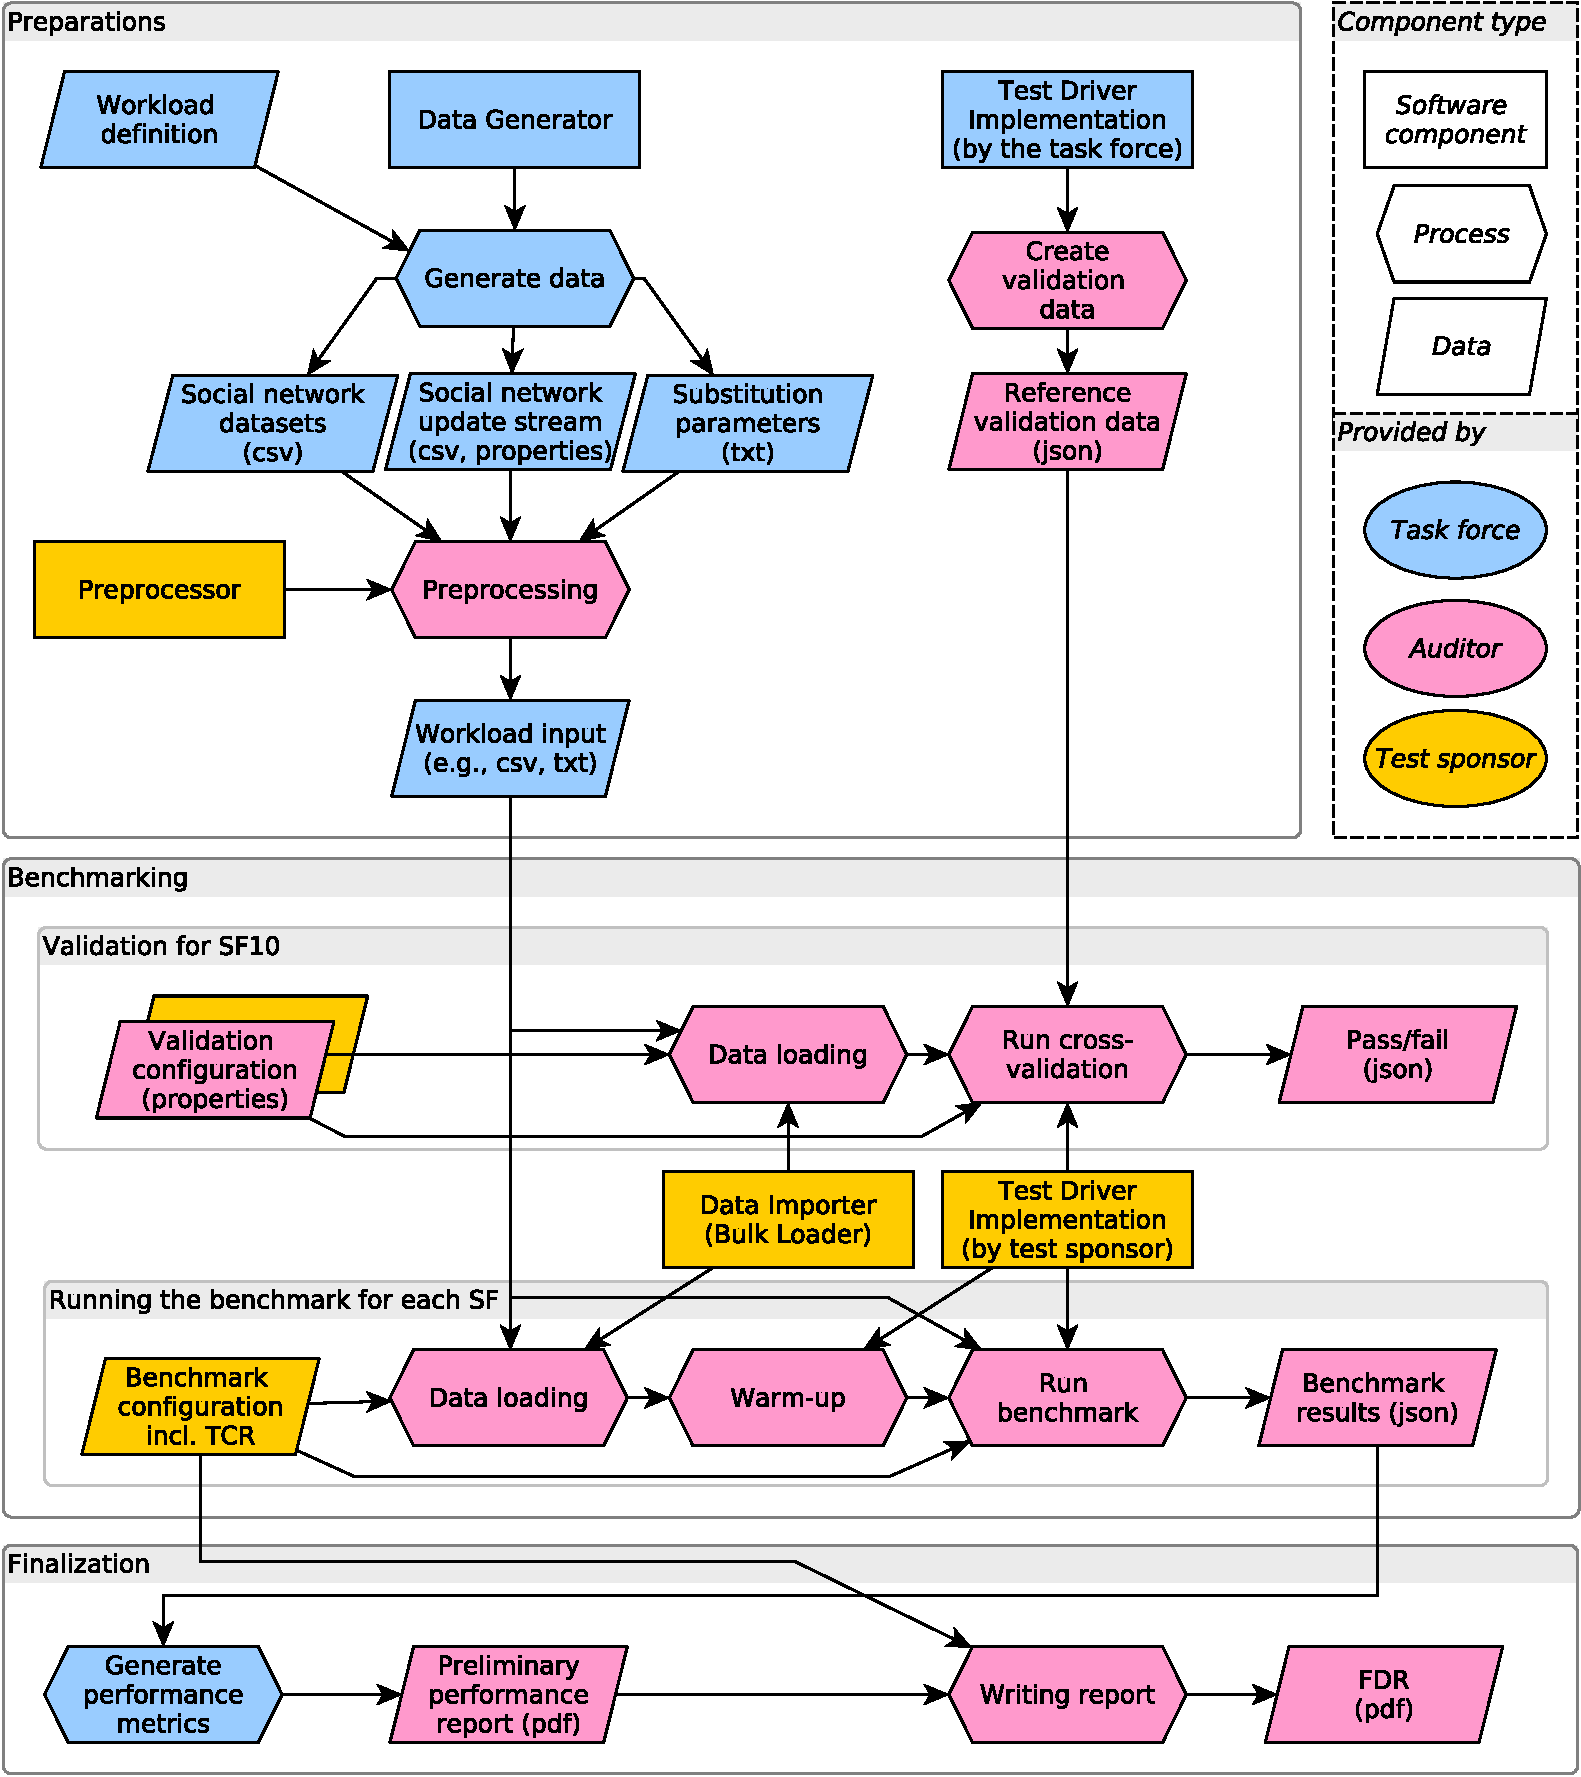
\includegraphics[scale=\yedscale]{figures/auditing-workflow}
    \caption{Benchmark execution and auditing workflow. For non-audited runs, the implementers perform the steps of the auditor.}
    \label{fig:audit-workflow}
\end{figure}

A key objective of the auditing guidelines for the Interactive workload is to \emph{allow a broad range of systems} to implement the benchmark.
Therefore, they do not impose constraints on the data model
(graph, relational, triple, \etc representations are allowed)
or on the query language
(both declarative and imperative languages are allowed).

\subsection{Scaling}
\label{sec:int-scaling}

\subsubsection{Scale Factors}

The scale factor of an SNB dataset is the size of the dataset in GiB of CSV (comma-separated values) files.
The size of a dataset is characterized by scale factors: SF10, SF30, SF100 \etc (see \autoref{sec:scale-factors}).
All datasets contain data for three years of social network activity.

The \emph{validation run} shall be performed on the SF10 dataset (see \autoref{sec:int-validation-data-set}). Note that the auditor may perform additional validation runs of the benchmark implementation using smaller datasets (\eg SF1) and issue queries.\footnote{%
An example test could be to issue complex reads with parameters such as \texttt{personId} and \texttt{messageId} selected from the \textsf{Person}/\textsf{Message} entities inserted from the update streams and cross-validate these against other systems. (The substitution parameters are taken from the initial snapshot of the graph so these nodes are not targeted by the regular workload executed by the driver.)%
}

Audited \emph{benchmark runs} of the Interactive workload shall use SF30 or larger datasets. The rationale behind this decision is to ensure that there is a sufficient number of update operations available to guarantee 2.5~hours of continuous execution (see \autoref{sec:int-measurement-window}).

% \begin{quote}
%     \emph{Rationale behind scaling.} The authors are aware that the prevalent practice for online benchmarks is to tie the reported throughput to the scale, \eg max 12.5 tpmC per warehouse in \mbox{TPC-C}. The authors depart from this practice here because with throughput tied to scale, test systems with interesting throughput rapidly become very expensive, raising the entry barrier for publishing a result. It is thought that scaling in buckets lowers the barrier of entry and reduces incentive to use hardware configurations that would be unusual in a production environment.
% \end{quote}
%COMMENTS FROM PAST GABOR TO FUTURE GABOR
%what it wants to say is that unlike TPC-C, you can get a large throughput (lots of ops) even on a small data set
%which is correct but we can ran out of updates due to the 2.5-hr simulation requirement
%so its (implied) conclusion does not hold fully hold for SNB interactive

\subsubsection{Social Network Datasets}
\label{sec:int-data-sets}

\paragraph{Initial dataset}
The dataset is divided into a bulk loadable initial database population (90\%) and an update stream (10\%). These are generated by the SNB data generator. The data generator has options for splitting the dataset into any number of files.

\paragraph{Dependencies between messages in the update stream}
The update stream contains the latest 10\% of the events in the simulated social network. These events form a single serializable sequence in time. Some events will depend on preceding events, for example a message must exist before a reply comment to the message is created. The data generator guarantees that these are separated by at least 10 seconds of simulation time.

\paragraph{Parallel updates}
The update stream may be broken into arbitrarily many sub-streams. The partition scheme is created by the \datagen. During benchmark execution, the driver preserves dependencies between update operations, such as ensuring not to refer to non-existent entities in updates (\eg a like is not added to a message which has not been inserted yet).

\subsection{Data Model and Data Loading}

\subsubsection{Supported Data Models}

SNB may be implemented with different data models (\eg relational, RDF, and different graph data models). The reference schema is provided in the specification using a UML-like notation. 


\subsubsection{Generated Input Data}
\label{sec:generated-data}

\paragraph{Storage}
The data generator produces comma-separated values (CSV) for all data models.

\paragraph{Data format}
A single attribute has a single data type, as follows:
\begin{description}
    \item [Identifier] This is an integer value foreign key or a URI in RDF. If this is an integer column, the implementation data type should support at least $2^{50}$ distinct values.
    \item [Date] A date should support a date range from 0000 to 9999 in the year field.
    \item [DateTime] A datetime should support a date range from 0000 to 9999 in the year field, with at least millisecond precision.
    \item [Short string] The string column for names may have a variable length and may have a declared maximum length, \eg 40 characters.
    \item [Long string] For example a message content may be a long string that is often short in the data but may not declare a maximum length and must support data sizes of up to 1~MB.
\end{description}

The above is stated in further detail in the benchmark specification, and it shall take precedence over the
above in the case of conflict.

A single attribute in the reference schema may not be divided into multiple attributes in the target schema.

\paragraph{Database schema}
A schema on the DBMS is optional. An RDF implementation for example may work without one. An RDF implementation is allowed to load the RDF reference schema and to take advantage of the data type and cardinality statements therein. 

\paragraph{Configuration parameters}
\datagen configuration parameters, including SF, distributions, number of persons, serialiser (\eg CsvSingularMergedFK) should be reported.

\paragraph{Primary data structures}
An RDF, relational, or graph schema may specify system specific options affecting DBMS storage layout. These may for example specify vertical partitioning. Vertical partitioning means anything from a column store layout with per-column allocated storage space to use of explicit column groups. Any mix of row or column-wise storage structures is allowed as long as this is declaratively specified on a per data structure-basis.

\paragraph{Auxiliary data structures}
Covering indices and clustered indices are allowed. If these are defined, then all replications of data implied by these must be maintained statement by statement, \ie each auxiliary data structure must be consistent with any other data structures of the table after each data manipulation operation.

A covering index is an index which materialises a specific order of a specific subset or possibly all columns of a table. 
A clustered index is an index which materialises all columns of a table in a specific order, which order may or may not be that of the primary key of the table. A clustered or covering index may be the primary or only representation of a table.

Any subset of the columns on a covering or clustered index may be used for ordering the data. A hash based index or a combination of a hash based and tree based index are all allowed, in row or column-wise or hybrid forms.

\paragraph{Loading the data}

We expect the SUT to provide some means to bulk load the data set either in the form of a dedicated offline loader component or an online loader that allows bulk inserting into a database.
The total of the bulk load time and the time for subsequent operations (indexing, computing statistics, \etc) must be reported in the FDR (see \autoref{sec:int-benchmark-workflow}).
As loading can be an expensive operation, it is allowed to conduct the audit such that the loading is only performend once, and the validation/benchmarking phases use the resulting database instance.
In practice, this can look like as follows:
(1)~load the data,
(2)~compute statistics, uniqueness constraints, keys, indices, \etc,
(3)~shut down the SUT,
(4)~create a backup of the database (\eg by copying the directory of the database).
For all subsequent runs, the databse shall be restored from the backup.

\subsection{Precomputation}

Precomputation of query results (both interim and end results) is allowed. However, systems must ensure that precomputed results (\eg materialized views) are kept consistent upon updates.

\subsection{Benchmark Software Components}
\label{sec:snb-software-components}
LDBC provides a test driver, data generator, and summary reporting scripts. Benchmark implementations shall use a stable version (\eg 0.3.6) of the test driver.

\subsubsection{Adaptation of the Test Driver to a DBMS}
\label{sec:test-driver}
A qualifying run must use a test driver that adapts the provided test driver to interface with the SUT. Such an implementation, if needed, must be provided by the test sponsor. The parameter generation, result recording, and workload scheduling parts of the test driver should not be changed. The auditor must be given access to the test driver source code used in the reported run.

The test driver produces the following artefacts for each execution as a by product of the run: Start and end timestamps in wall clock time, recorded with microsecond precision. The identifier of the operation and any substitution parameters.


\subsubsection{Summary of Benchmark Results}
\label{sec:performance-metrics}
A separate test summary tool provided with the test driver analyses the test driver log(s) after a measurement window is completed. 

The tool produces for each of the distinct queries and transactions the following summary:
\begin{itemize}
    \item Run time of query in wall clock time.
    \item Count of executions.
    \item Minimum/mean/percentiles/maximum execution time.
    \item Standard deviation from the average execution time.
\end{itemize}
The tool produces for the complete run the following summary:
\begin{itemize}
    \item Operations per second for a given SF (throughput). This is the primary metric of this workload.
    \item The total execution time in wall clock time.
    \item The total number of completed operations.
\end{itemize}


\subsection{Implementation Language and Data Access Transparency}

The queries and updates may be implemented in a domain-specific query language or as procedural code written in a general-purpose programming language (\eg using the API of the database).

\subsubsection{Implementations Using a Domain-Specific Query Language}
\label{sec:snb-domain-specific-query-language}

If a domain-specific query language is used, \eg SPARQL, SQL, Cypher, or Gremlin, then explicit query plans are prohibited in all the read-only queries.%
\footnote{If the queries are not clearly declarative, the auditor must ensure that they do not specify explicit query plans by investigating their source code and experimenting with the query planner of the system (\eg using SQL's \texttt{EXPLAIN} command).}
The update transactions may still consist of multiple statements, effectively amounting to explicit plans.

Explicit query plans include but are not limited to:
\begin{itemize}
    \item Directives or hints specifying a join order or join type
    \item Directives or hints specifying an access path, \eg which index to use
    \item Directives or hints specifying an expected cardinality, selectivity, fanout or any other information that pertains to the expected number or results or cost of all or part of the query.
\end{itemize}

\begin{quote}
    \emph{Rationale behind the applied restrictions.} The updates are effectively OLTP and, therefore, the customary freedoms apply, including the use of stored procedures, however subject to access transparency. Declarative queries in a benchmark implementation should be such that they could plausibly be written by an application developer. Therefore, their formulation should not contain system specific aspects that an application developer would be unlikely to know. In other words, making a benchmark implementation should not require uncommon sophistication on behalf of the developer. This is regular practice in analytical benchmarks, \eg \mbox{TPC-H}.
\end{quote}

\subsubsection{Implementations Using a General-Purpose Programming Language}
\label{sec:snb-general-purpose-programming-language}

Implementations using a general-purpose programming language for specifying the queries (including procedural, imperative, and API-based implementations) are expected to respect the rules described in \autoref{sec:query-languages}.
For these implementations, the rules in \autoref{sec:snb-domain-specific-query-language} do not apply.

\subsection{Correctness of Benchmark Implementation}

\subsubsection{Validation data set}
\label{sec:int-validation-data-set}
The scale factor 10 shall be used as validation data set.

\subsubsection{ACID Compliance}
\label{sec:int-acid-compliance}

The Interactive workload requires full ACID support (\autoref{sec:acid-compliance}) from the SUT.
This is tested using the LDBC ACID test suite.
For the specification of this test suite, see \autoref{sec:acid-test-suite} and the related software repository at \url{https://github.com/ldbc/ldbc_acid}.

\paragraph{Expected level of isolation}
If a transaction reads the database with intent to update, the DBMS must guarantee that repeating the same read within the same transaction will return the same data. This also means that no more and no less data rows must be returned. In other words, this corresponds to snapshot or to serializable isolation. If the database is accessed without transaction context or without intent to update, then the DBMS should provide read committed semantics, \eg repeating the same read may produce different results but these results may never include effects of pending uncommitted transactions.

\paragraph{Durability and checkpoints}

A checkpoint is defined as the operation which causes data persisted in a transaction log to become durable outside of the transaction log. Specifically, this means that an SUT restart after instantaneous failure following the completion of the checkpoint may not have recourse to transaction log entries written before the end of the checkpoint.

A checkpoint typically involves a synchronisation barrier at which all data committed prior too the moment is required to be in durable storage that does not depend on the transaction log.
Not all DBMSs use a checkpointing mechanism for durability. For example a system may rely on redundant storage of data for durability guarantees against instantaneous failure of a single server.

The measurement window may contain a checkpoint. If the measurement window does not contain one, then the restart test will involve redoing all the updates in the window as part of the recovery test.

The timed window ends with an instantaneous failure of the SUT. Instantaneously killing all the SUT process(es) is adequate for simulating instantaneous failure. All these processes should be killed within one second of each other with an operating system action equivalent to the Unix \verb+kill -9+. If such is not available, then powering down each separate SUT component that has an independent power supply is also possible.

The restart test consists of restarting the SUT process(es) and finishes when the SUT is back online with all its functionality and the last successful update logged by the driver can be seen to be in effect in the database.
%In the case of a distributed (scale-out) system, a particular partition may be recovered whereas another one is still in the process of recovering. If this is so, then checking for the last update shall not be done until all partitions are online.

If the SUT hardware was powered down, the recovery period does not include the reboot and possible file system check time. The recovery time starts when the DBMS software is restarted.




\paragraph{Recovery} 
The SUT is to be restarted after the measurement window and the auditor will verify that the SUT contains the entirety of the last update recorded by the test driver(s) as successfully committed. The driver or the implementation have to make this information available.

Once an official run has been validated, the recovery capabilities of the system must be tested. The system and the driver must be configured in the same way as in during the benchmark execution. After a warm-up period, an execution of the benchmark will be performed under the same terms as in the previous measured run.

\paragraph{Measuring recovery time}
At an arbitrary point close to 2 hours of wall clock time during the run, the machine will be shut down. Then, the auditor will restart the database system and will check that the last committed update (in the driver log file) is actually in the database. The auditor will measure the time taken by the system to recover from the failure. Also, all the information about how durability is ensured must be disclosed. If checkpoints are used, these must be performed with a period of 10 minutes at most.


\subsection{Benchmarking Workflow}
\label{sec:int-benchmark-workflow}

A benchmark execution is divided into the following processes (these processes are also shown in \autoref{fig:audit-workflow}):

\begin{description}
    \item[Generate data] This includes running the data generator, placing the generated files in a staging area, configuring storage, setting up the SUT configuration and preparing any data partitions in the SUT. This may include preallocating database space but may not include loading any data or defining any schema having to do with the benchmark. The \verb|ldbc.snb.interactive.update_interleave| driver parameter must come from the \verb|updateStream.properties| file, which is created by the data generator. That parameter should never be set manually. This parameter signifies the average distance of update operations in the workload.
    \item[Preprocessing] If needed, the output from the data generator is converted to a format that is loadable by the test-specific implementation of the data importer.
    \item[Create validation data] Using one of the reference implementations of the benchmark, the reference validation data is obtained in .json format.
    \item[Data loading] The test sponsor must provide all the necessary documentation and scripts to load the dataset into the database to test.
    This includes defining the database schema, if any, loading the initial database population, making this durably stored and gathering any optimiser statistics.
    The system under test must support the different data types needed by the benchmark for each of the attributes at their specified precision. No data can be filtered out, everything must be loaded. The test sponsor must provide a tool to perform arbitrary checks of the data or a shell to issue queries in a declarative language if the system supports it.
    \item[Run cross-validation] This step uses the data loader to populate the database, but the load is not timed. The validation data set is used to verify the correctness of the SUT. The auditor must load the provided dataset and run the driver in validation mode, which will test that the queries provide the official results.  The benchmarking workflow will not go beyond this point unless results match the expected output.
    \item[Warm-up] Benchmark runs are preceded by a warm-up which must be performed using the LDBC driver.
    \item[Run benchmark] The bulk load time is reported and is equal to the amount of elapsed wall clock time between starting the schema definition and receiving the confirmation message of the end of statistics gathering. The workflow runs begin after the bulk load is completed. If the run does not directly follow the bulk load, it must start at a point in the update stream that has not previously been played into the database. In other words, a run may only include update events whose timestamp is later than the latest message creation date in the database prior to start of run. The run starts when the first of the test drivers send its first message to the SUT. If the SUT is running in the same process as the driver, the window starts
    when the driver starts. Also, make sure that the \verb|-rl/--results_log| is enabled. Make sure that all operations are enabled and the frequencies are those for the selected scale factor (see the exact specification of the frequencies in the specification appendix B.1. Scale Factor Statistics for the Interactive Workload).
\end{description}

\subsubsection{Query Timing During Benchmark Run}
\label{sec:ontime-requirements}
A valid benchmark run must last at least 2 hours of wall clock time.
In order to be valid, a benchmark run needs to meet the ``95\% on-time requirement''.
The \texttt{results\_log.csv} file contains the $\mathsf{actual\_start\_time}$ and the $\mathsf{scheduled\_start\_time}$ of each of the issued queries. In order to have a valid run, 95\% of the queries must meet the following condition:
\begin{equation*}
\mathsf{actual\_start\_time} - \mathsf{scheduled\_start\_time} < 1\
\mathrm{second}
\end{equation*}

If the execution of the benchmark is valid, the auditor must retrieve all the files from directory specified by \verb|--results_dir| which includes configuration settings used, results log and results summary. All of which must be disclosed.

\subsubsection{Measurement Window}
\label{sec:int-measurement-window}

Benchmark runs execute the workload on the SUT in two phases (\autoref{fig:measurement-window-selection}).
First, the SUT must undergo a warm-up period that takes at least 30 minutes. The goal of this is to put the system in a steady state which reflects how it would behave in a normal operating environment. The performance of the operations during warm-up is not considered.
Next, the SUT is benchmarked during a two-hour measurement window. Operation times are recorded and checked to ensure the ``95\% on-time requirement'' is satisfied.

\begin{figure}[h]
    \centering
    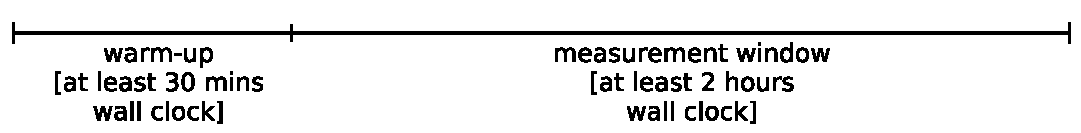
\includegraphics[width=.7\linewidth]{figures/measurement-window-selection}
    \caption{Warm-up and measurement window for benchmark run.}
    \label{fig:measurement-window-selection}
\end{figure}

The SNB \datagen produces 3~years worth data of which 10\% is used for updates (\autoref{sec:int-data-sets}), \ie approximately $3 \times 365 \times 0.1 = 109.5~\text{days} = 2628~\text{hours}$.
To ensure that the 2.5~hour wall clock period has enough input data, the lower bound of TCR is defined as 0.001 (if $2628$ hours of updates are played back at more than $1000\times$ speed, the benchmark framework runs out of updates to execute). System that can achieve a better compression (\ie lower TCR value) on a given scale factor should use larger SFs for their benchmark runs -- otherwise their total runs will be less than 2.5~hours, making them unsuitable for auditing.

%The test summary tool may be used for reading the logs created by a test driver.

\subsection{Full Disclosure Report}
\label{sec:int-fdr}

Upon successful completion of the audit, an FDR is compiled. In addition to the general requirements, the full disclosure shall cover the following:

\begin{itemize}
    \item General terms: an executive summary and declaration of the credibility of the audit
    \item System description and pricing summary: see \autoref{sec:system-config}
    \item Data generation and data loading: see \autoref{sec:generated-data}
    \item Test driver details: see \autoref{sec:test-driver}
    \item Performance metrics: see \autoref{sec:performance-metrics}
    \item Validation results: see \autoref{sec:int-validation-data-set}
    \item ACID compliance: see \autoref{sec:acid-compliance}
    \item List of supplementary materials
\end{itemize}

To ensure reproducibility of the audited results, a supplementary package is attached to the full disclosure report. This package should contain:

\begin{itemize}
    \item A README file with instructions specifying how to set up the system and run the benchmark
    \item Configuration files of the database, including database-level configuration such as buffer size and schema descriptors (if necessary)
    \item Source code or binary of a generic driver that can be used to interact with the DBMS
    \item SUT-specific LDBC driver implementation (similarly to the projects in \url{https://github.com/ldbc/ldbc_snb_interactive_impls})
    \item Script or instructions to compile the LDBC Java driver implementation
    \item LDBC configuration files (\texttt{.properties}), including the \texttt{time\_compression\_ratio} values used in the audited runs
    \item Scripts to preprocess the input files (if necessary) and to load the data sets into the database
    \item Scripts to create validation data sets and to run the benchmark
    \item The implementations of the queries and the update operations, including their complete source code (\eg declarative queries specifications, stored procedures, \etc)
    \item Implementation of the ACID test suite
    \item Binary package of the DBMS (\eg \texttt{.deb} or \texttt{.rpm})
\end{itemize}



%%%%%%%%%%%%%%%%%%%%%%%%%%%%%%%%%%%%%%%%%%%%%%%%%%%%%%%%%%%%%%%%%%%%%%%%%%%%%%
%%%%%%%%%%%%%%%%%%%%%%%%%%%%%%%%%%%%%%%%%%%%%%%%%%%%%%%%%%%%%%%%%%%%%%%%%%%%%%
%%%%%%%%%%%%%%%%%%%%%%%%%%%%%%%%%%%%%%%%%%%%%%%%%%%%%%%%%%%%%%%%%%%%%%%%%%%%%%

\section{Auditing Rules for the Business Intelligence Workload}
\label{sec:bi-workload-audit}

%%%%%%%%%%%%%%%%%%%%%%%%%%%%%%%%%%%%%%%%%%%%%%%%%%%%%%%%%%%%%%%%%%%%%%%%%%%%%%
%%%%%%%%%%%%%%%%%%%%%%%%%%%%%%%%%%%%%%%%%%%%%%%%%%%%%%%%%%%%%%%%%%%%%%%%%%%%%%
%%%%%%%%%%%%%%%%%%%%%%%%%%%%%%%%%%%%%%%%%%%%%%%%%%%%%%%%%%%%%%%%%%%%%%%%%%%%%%

A key objective of the auditing guidelines for the BI workload is to \emph{allow a broad range of systems} to implement the benchmark.
Due to the BI workload's analytical nature, we expect not only DBMSs but also analytical tools which operate on read-only data (stored \eg in HDFS or in an object store).
Therefore, they do not impose constraints on transactional guarantees.

\subsection{Scaling}
\label{sec:bi-scaling}

Audited \emph{benchmark runs} of the BI workload shall use SF30 or larger datasets.
The rationale behind this decision is to ensure that there is a sufficient number of update operations available to guarantee the execution during the duration of the measurement window (see \autoref{sec:bi-benchmark-workflow}).

\subsection{Query Declarativity}
\label{sec:bi-query-declarativity}

Systems should use a domain-specific query language (\eg Cypher, Gremlin, GSQL) for the implementation.
General-purpose programming languages (\eg C, C\texttt{++}, Java, Julia) are not allowed.

Implementations shall not use \emph{query-specific stored procedures written in a general-purpose programming language} (\eg a given procedure which implements BI Q5).
Using the stored procedure libraries considered to be the ``standard libraries'' of the SUT is allowed. (These libraries often include features such as weighted shortest path algorithms.)
Implementations may use \emph{stored procedures written in a domain-specific language}.

The auditor's responsibility is to enforce this requirement, \ie they should verify whether query implementations only use the following implementation techniques:
\begin{enumerate}
    \item the domain-specific language of the SUT,
    \item the SUT's standard stored procedure library or libraries, and
    \item stored procedures written in a domain-specific language,
\end{enumerate}

\subsection{Query Variants}
\label{sec:bi-query-variants}

Several queries (\eg \queryRefCard{bi-read-14}{BI}{14}) use (A) and (B) variants with different sets of input parameters.
These should be run in a mix and the SUT should not receive any hints on which variant it is currently evaluating (\eg Q14(A) or Q14(B)).
Moreover, it is not allowed for the query implementations to contain code that aims to detect the query variant used.

\subsection{Benchmark Workflow}
\label{sec:bi-benchmark-workflow}

\begin{figure}[htbp]
    \centering
    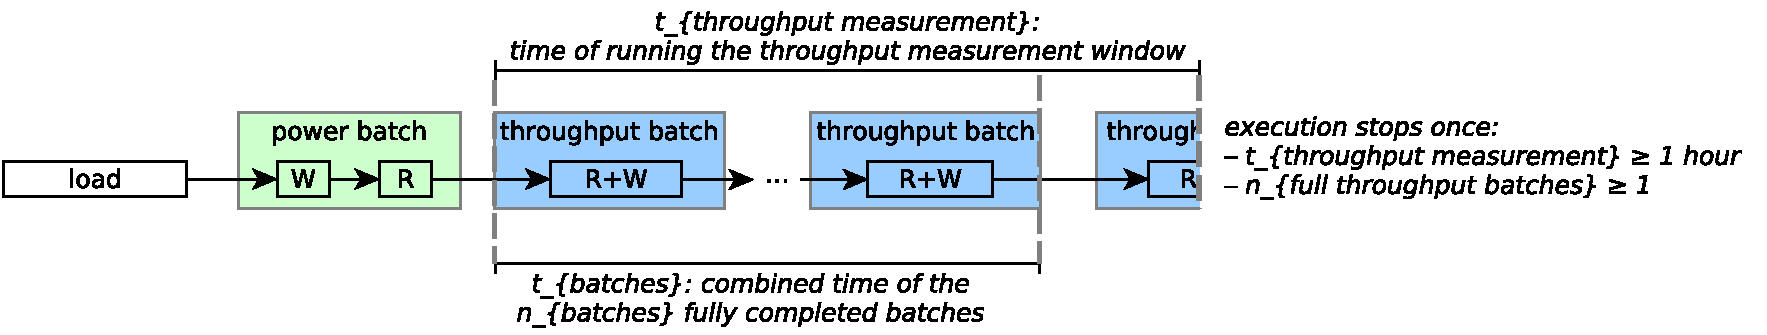
\includegraphics[scale=\yedscale]{figures/bi-auditing-workflow.pdf}
    \caption{BI auditing workflow.}
    \label{fig:bi-auditing-workflow}
\end{figure}

The BI workflow (\autoref{fig:bi-auditing-workflow}) consists of three parts.

\begin{itemize}
    \item \textbf{Loading} the data set.
    \item Running the \textbf{power test}, \ie apply one day's write batch and run the reads sequentially.
    \item Running the \textbf{throughput test}, \ie run batches of (potentially) concucrrent write operations (applying one day's worth of data per batch) and read queries.
    The execution of this test is called the \emph{throughput measurement window}, which should
    run at least for 2 hours and
    include at least one fully completed batch.
\end{itemize}

The runtimes should be reported as follows:
\begin{itemize}
    \item The \emph{load time} ($t_\textit{load}$) denotes the time to load the data into the SUT and initialize auxiliary data structures (if applicable).
    \item The \emph{power test time} ($t_\textit{power test}$) denotes the time to perform the power test.
    \item The \emph{throughput measurement window time} ($t_\textit{throughput\ measurement}$) denotes the time to perform the throughput test, including potentially unfinished batches.
    \item The \emph{full throughput batches time} ($t_\textit{full\ throughput\ batches}$) denotes the time to evaluate the fully completed batches during the throughput measurement window.
\end{itemize}

Note that a ``warm-up'' period is not allowed (unlike the Interactive workload where such a period is required, see \autoref{sec:int-measurement-window}).

\subsection{Target Metric}
\label{sec:bi-target-metric}

The performance of the SUT is characterized by the \emph{number of batches executed per day} ($\mathit{bpd}$).

During the measurement window, the benchmark runs a sequence of throughput batches for a total of $t_\textit{throughput\ measurement}$ time ($n_\textit{full\ throughput\ batches} \geq 1$ and $t_\textit{throughput\ measurement} \geq 2\text{ hours}$).
Then, the number of fully completed batches
$n_\textit{full\ throughput\ batches}$
and the time required to run them
$t_\textit{full\ throughput\ batches}$
are determined.
Using these, the metric is defined as:
$$
\mathit{bpd} = (24 - t_\textit{load}) \times \frac{n_\textit{full\ throughput\ batches}}{t_\textit{full\ throughput\ batches}}
$$

For example, if the SUT took $3.5\texttt{ hours}$ to load, executed the fully completed throughput batches for $1.75$ hours and completed $7$ batches:
$$
\mathit{bpd} = (24 - 3.5) \times \frac{7}{1.75} = 82\text{ batches/day}
$$

\subsection{Implementation Rules}
\label{sec:bi-implementation-rules}

\subsubsection{Correctness}
\label{sec:bi-correcntess}
The SUT shall evaluate all operators correctly.
The validation of correctness is performed on the output of the \emph{power test} step.
The rationale for using this step is that during concurrent execution of R/W operations in the \emph{throughput test}, it is not possible to guarantees deterministic query results, making validation impossible. Moreover, this step already includes a write batch, therefore the query results indirectly test the correctness of the implementation of write operations.

\subsubsection{Auxiliary Data Structures}
\label{sec:bi-auxiliary-data-structures}
Using auxiliary data structures (\eg indexes, materialized views) is allowed if they are kept in an up-to-date state after each write operation.

\subsubsection{Transactional Features}
\label{sec:bi-transactional-features}
We allow two categories of systems to compete on the benchmark.
These systems compete on the same leaderboard but have slightly different implementation rules.

\begin{itemize}
    \item \emph{Purely analytical systems} do not support concurrent reads and writes, or they do not make use of them in their \snbbi implementation.
    \item \emph{Transaction-capable systems} makes use of concurrent reads and writes.
\end{itemize}

\emph{Purely analytical systems} shall perform their \emph{throughput batches} in two steps:
first, they should perform the writes (refresh operations),
then, they should perform the reads (queries).
For such systems, passing the \emph{ACID compliance test} is not required.

\emph{Transaction-capable systems} are allowed to run concurrent read and write operations in their \emph{throughput batches}.
These systems should guarantee at least \emph{TODO} isolation level and guarantee \emph{ACID compliance} (\autoref{sec:acid-compliance}).

\subsection{Full Disclosure Report}
\label{sec:bi-fdr}

The \emph{full disclosure report} (FDR) and the \emph{supplementary package} shall contain
the same information as for SNB Interactive (\autoref{sec:int-fdr}),
including, if applicable (\autoref{sec:bi-implementation-rules}), the ACID compliance report (\autoref{sec:acid-compliance}).
